\documentclass[letterpaper,11pt,openany,oneside]{book}
% package includes
\usepackage{titlepic}
\usepackage{graphicx}
\usepackage{hyperref}
% define the title
\author{CW2 Peter Goodspeed-Niklaus}
\title{HH-60 DA 2408-17 Photo Guide}
\titlepic{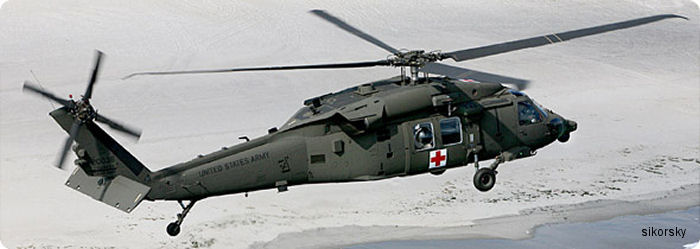
\includegraphics[width=\textwidth]{Images/hh-60m.jpg}}
% document options
\pagestyle{headings}
\begin{document}
\frontmatter
% generates the title
\maketitle
\clearpage
\setcounter{page}{1}
\chapter*{About This Document}
Indices are identical but for ordering. First index is ordered per the part number on a reference DA~2408-17. Second index is ordered alphabetically by nomenclature.

This document was generated in \LaTeXe. Source files may be found at \url{https://www.github.com/INSERT URL HERE}. Fork the project for changes; pull requests will not be accepted. Tools used authoring this document include \href{http://texstudio.sourceforge.net/}{TeXstudio}, \href{http://miktex.org/}{MiKTeX}, and \href{http://johnmacfarlane.net/pandoc/}{Pandoc}.

For further information, reference TM 1-1520-237-23-9, Appendix~C: Aircraft Master Inventory Guide.
\mainmatter
\chapter*{Index, DA~2408-17 Ordering}
\section*{Section I: Cockpit}
the whole damn avionics compartment \ref{avionics}
\section*{Section II: Cabin}
bar
\section*{Section III: Transition Section}
bat
\section*{Section IV: Tail Cone}
baz
\section*{Section V: Tail Rotor Pylon}
bim
\chapter*{Index, Alphabetical by Nomenclature}
\section*{Section I: Cockpit}
foo
\section*{Section II: Cabin}
bar
\section*{Section III: Transition Section}
bat
\section*{Section IV: Tail Cone}
baz
\section*{Section V: Tail Rotor Pylon}
bim
\chapter*{Figures}
\begin{figure}[htp]
	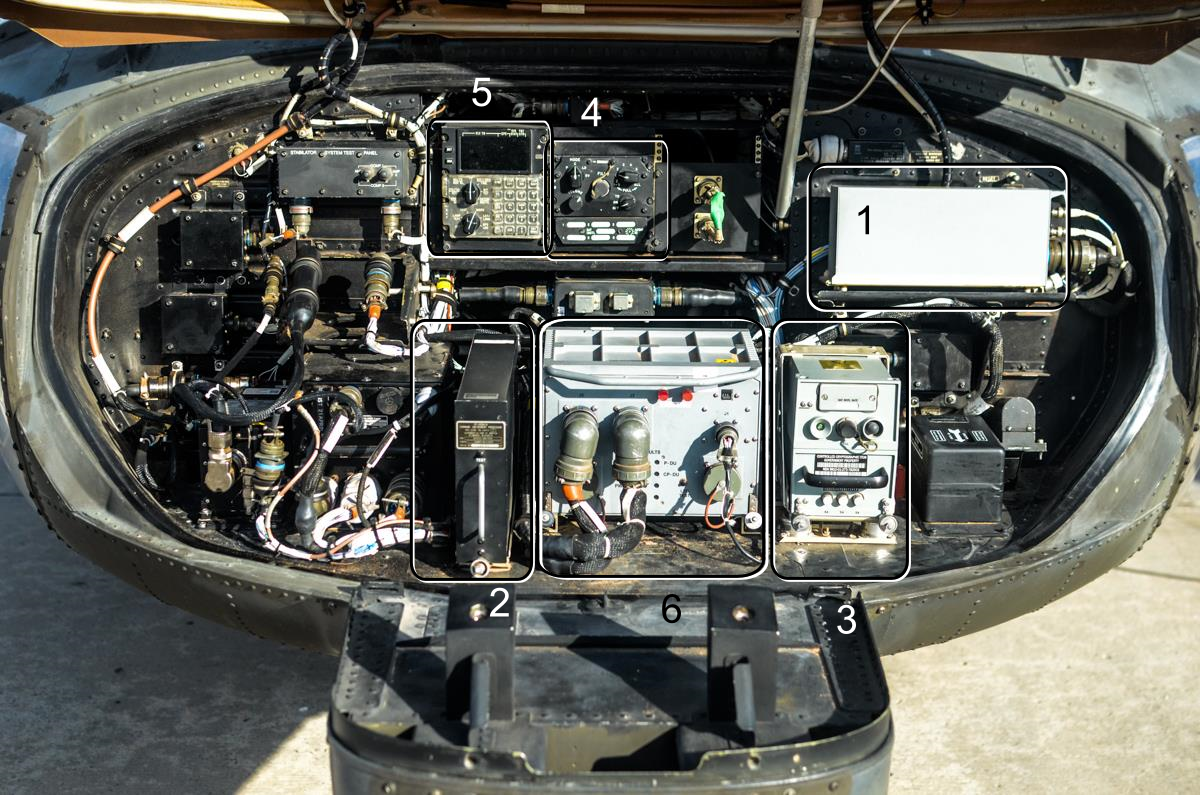
\includegraphics[width=\textwidth]{Images/avionics-bay.jpg}
	\caption{Avionics Bay} \label{avionics}
\end{figure}
\end{document}
